\anexo{Brainstorming: material y transcripción de la sesión}
\label{anx:brainstorming}

Este anexo presenta el material de la sesión de brainstorming del 10 de octubre de 2026, descripta en la Sección~\ref{sec:brainstorming}: los acercamientos fotográficos a la matriz impacto/esfuerzo, la tabla completa de las ideas que pasaron a la matriz y la transcripción de la sesión. Los participantes se identifican con un código: B01, Juan Ignacio Gonzalez (DevOps); B02, Braulio Jauregui (desarrollador backend); B03, Diego Dangona (Product Manager); B04, Agostina Targarico (Marketing); y B05, Gabriel Aran (desarrollador backend).

\section*{\thechapter.1 Acercamientos a la matriz}
\addcontentsline{toc}{subsection}{\thechapter.1 Acercamientos a la matriz}

La matriz completa se presenta en la Figura~\ref{fig:brainstorming-matriz-completa} de la Sección~\ref{sec:brainstorming-resultados}. Las Figuras~\ref{fig:brainstorming-sector-poco} y~\ref{fig:brainstorming-sector-mucho} muestran de cerca sus dos mitades, con el texto de cada idea legible.

\begin{figure}[ht]
    \centering
    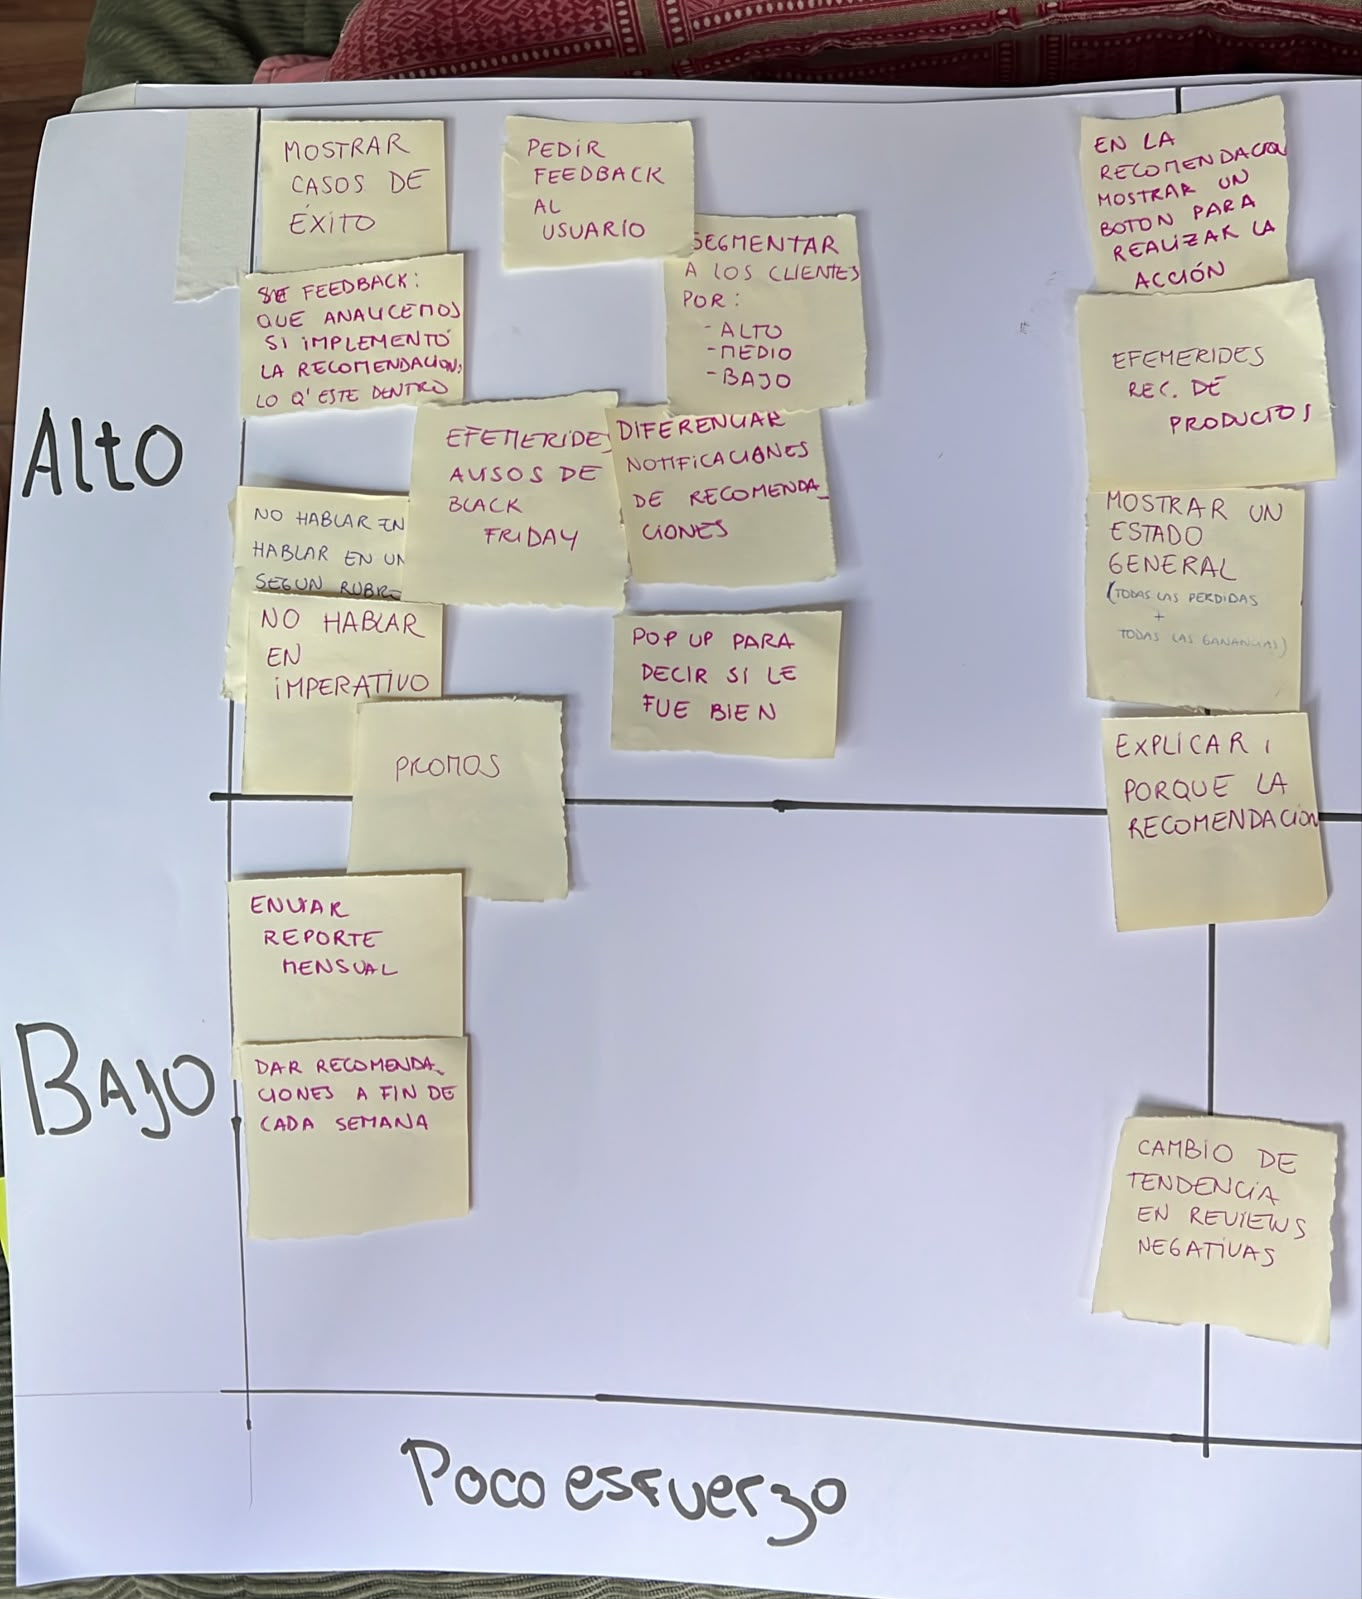
\includegraphics[width=0.85\textwidth]{./images/brainstorming-2.jpeg}
    \caption{Acercamiento al sector de poco esfuerzo: ideas en los cuadrantes alto-poco esfuerzo y bajo-poco esfuerzo. Sesión del 10 de octubre de 2026.}
    \label{fig:brainstorming-sector-poco}
\end{figure}

\noindent\textit{Fuente: elaboración propia.}

\FloatBarrier

\begin{figure}[ht]
    \centering
    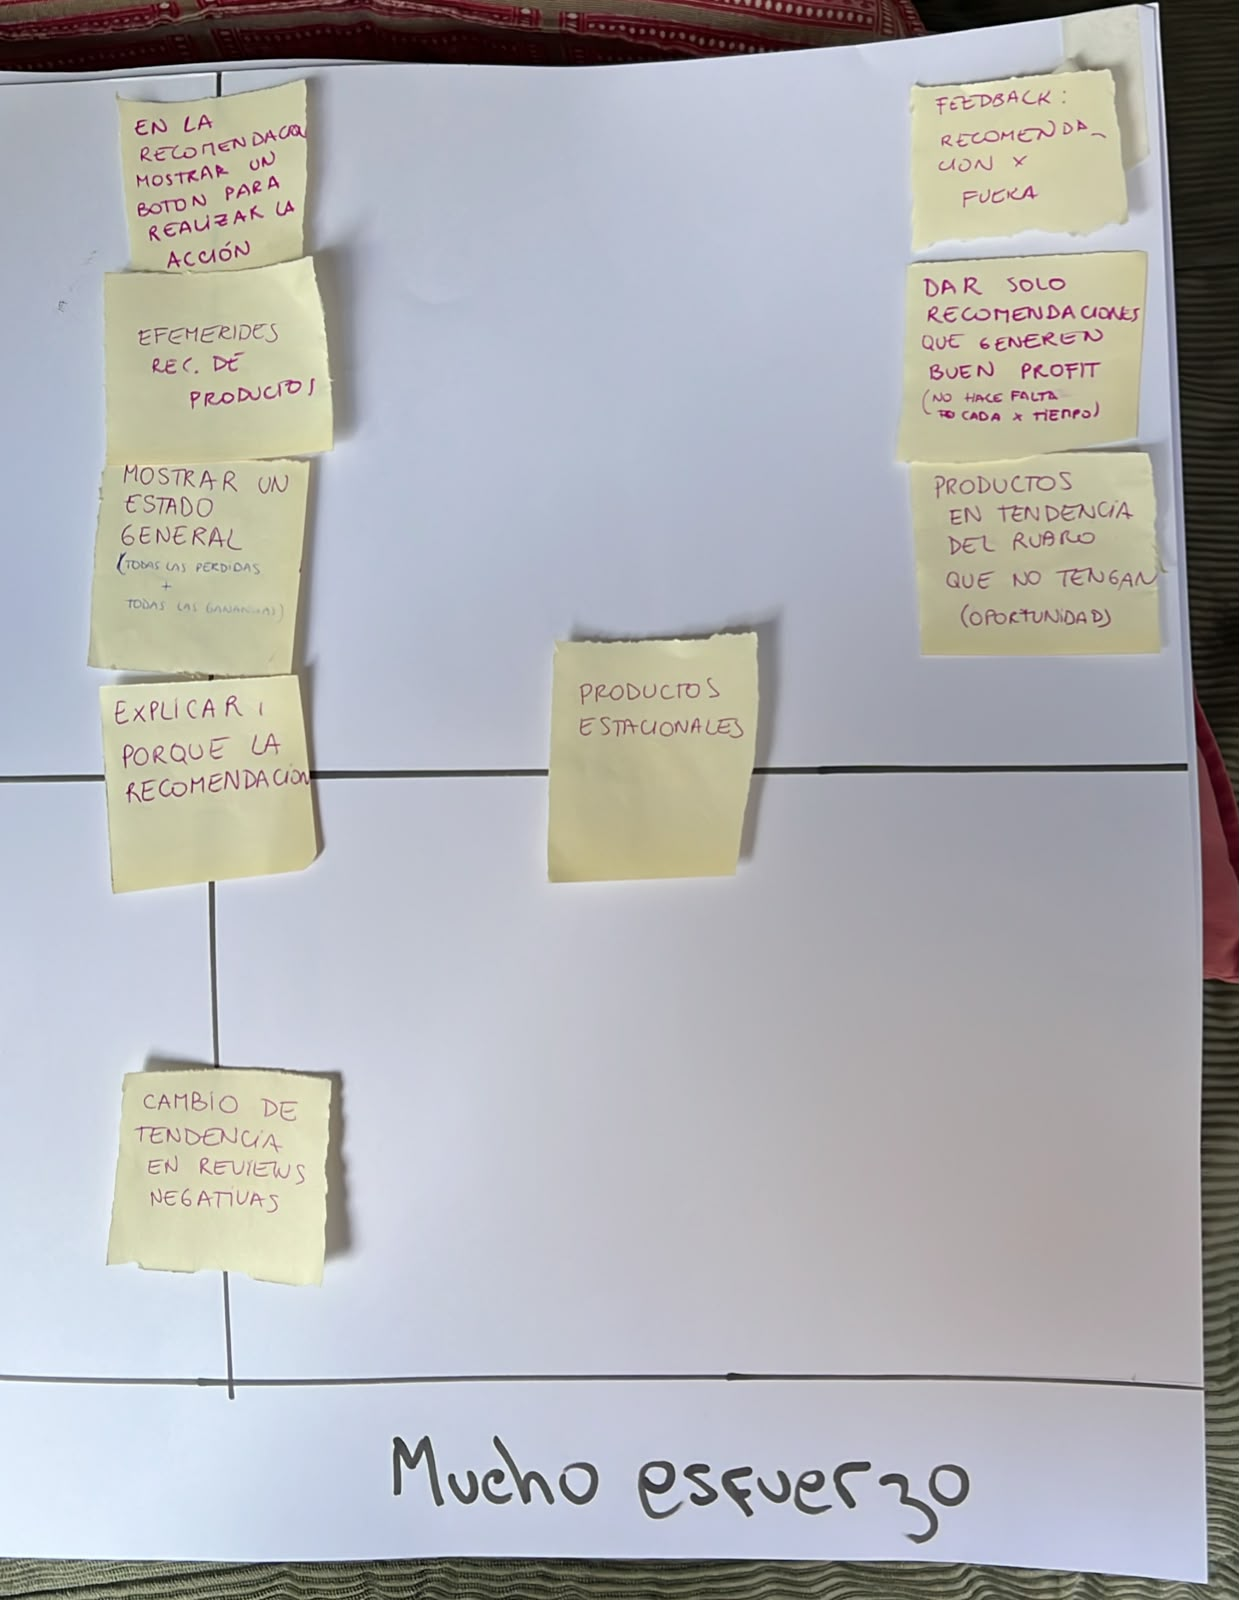
\includegraphics[width=0.75\textwidth]{./images/brainstorming-1.jpeg}
    \caption{Acercamiento al sector de mucho esfuerzo: ideas en los cuadrantes alto-mucho esfuerzo y bajo-mucho esfuerzo. Sesión del 10 de octubre de 2026.}
    \label{fig:brainstorming-sector-mucho}
\end{figure}

\noindent\textit{Fuente: elaboración propia.}

\FloatBarrier

\section*{\thechapter.2 Ideas más votadas en la matriz}
\addcontentsline{toc}{subsection}{\thechapter.2 Ideas más votadas en la matriz}

La Tabla~\ref{tab:brainstorming-ideas} presenta los 21 grupos de ideas más votados que pasaron a la matriz, con su cuadrante y su estado de implementación al cierre del proyecto.

{\small
\begin{longtable}{>{\raggedright\arraybackslash}p{5cm} >{\raggedright\arraybackslash}p{2.6cm} >{\raggedright\arraybackslash}p{6.4cm}}
\caption{Ideas más votadas de la sesión de brainstorming y estado de implementación.}
\label{tab:brainstorming-ideas}\\
\hline
\textbf{Idea} & \textbf{Cuadrante} & \textbf{Estado} \\
\hline
\endfirsthead
\multicolumn{3}{l}{\textit{Continuación de la Tabla~\thetable}} \\
\hline
\textbf{Idea} & \textbf{Cuadrante} & \textbf{Estado} \\
\hline
\endhead
\hline
\endfoot
\multicolumn{3}{l}{\textit{Ideas que validan el diseño implementado}} \\
\hline
Pedir feedback al usuario & Alto / poco esfuerzo & Implementada: marcar como ejecutada, deshacer, «No fui yo» (HU-07). \\
Efemérides: avisos de fechas clave (Black Friday, Día de la Madre) & Alto / poco esfuerzo & Implementada: recomendación de fecha clave con calendario por rubro (HU-06). \\
Efemérides: qué productos promocionar & Alto / mucho esfuerzo & Implementada: fecha clave sobre los productos más vendidos de los últimos 28 días. \\
Promos & Alto / poco esfuerzo & Implementada: rotación en caída y fechas clave sugieren promociones. \\
Segmentar clientes en alto, medio y bajo & Alto / poco esfuerzo & Implementada: segmentación RFM con \emph{k}-means y CLV (HU-10). \\
Explicar por qué la recomendación & Alto / mucho esfuerzo & Implementada: campo «Por qué te lo recomendamos» y explicación de la priorización en el detalle. \\
Productos estacionales & Medio / mucho esfuerzo & Implementada: pronóstico Holt-Winters con estacionalidad y preparación anticipada (HU-02). \\
Mostrar casos de éxito & Alto / poco esfuerzo & Implementada: vista de impacto esperado versus real (HU-08). \\
Detectar si el emprendedor implementó la recomendación & Alto / poco esfuerzo & Implementada: inferencia automática de la ejecución a partir de snapshots de stock y precio (HU-07). \\
\hline
\multicolumn{3}{l}{\textit{Ideas parcialmente implementadas o incorporadas a partir de la sesión}} \\
\hline
Diferenciar notificaciones de recomendaciones & Alto / poco esfuerzo & Implementada a partir de la sesión: notificaciones separadas de las recomendaciones (RF-22). \\
Pop-up para preguntar si le sirvió & Alto / poco esfuerzo & Parcial: impacto medido automáticamente; falta consulta activa al emprendedor. \\
Botón para realizar la acción desde la tarjeta & Alto / mucho esfuerzo & Parcial: CTA en cada tarjeta; sin integración de escritura hacia la plataforma (trabajo futuro: «acciones con un clic»). \\
Dar solo recomendaciones que generen buen margen & Alto / mucho esfuerzo & Parcial: el bandit prioriza lo que funcionó; falta filtro por margen (requiere el costo del producto). \\
No hablar en imperativo & Alto / poco esfuerzo & Parcial: el LLM redacta los mensajes; aplicación efectiva depende del \emph{system prompt} de Gemini. \\
Adaptar el tono al rubro & Alto / poco esfuerzo & Parcial: el LLM recibe el rubro como contexto; aplicación efectiva depende del \emph{system prompt} de Gemini. \\
\hline
\multicolumn{3}{l}{\textit{Trabajo futuro o descartadas}} \\
\hline
Mostrar un estado general (pérdidas y ganancias acumuladas) & Alto / mucho esfuerzo & Trabajo futuro: viable solo como impacto acumulado de recomendaciones ejecutadas. \\
Feedback de acciones ejecutadas fuera de la plataforma & Alto / mucho esfuerzo & Trabajo futuro: no observable desde la API de la plataforma. \\
Productos en tendencia del rubro que la tienda no tiene & Alto / mucho esfuerzo & Trabajo futuro: requiere fuentes de datos de mercado externas, fuera del alcance actual. \\
Enviar reporte mensual & Bajo / poco esfuerzo & Trabajo futuro: bajo impacto percibido en la matriz. \\
Dar recomendaciones al cierre de cada semana & Bajo / poco esfuerzo & Trabajo futuro: bajo impacto percibido en la matriz. \\
Cambio de tendencia en reseñas negativas & Bajo / mucho esfuerzo & Descartada: la API de Tiendanube no expone reseñas de forma nativa; impacto bajo. \\
\end{longtable}
}

\noindent\textit{Fuente: elaboración propia a partir de los resultados de la sesión del 10 de octubre de 2026.}

\FloatBarrier

\section*{\thechapter.3 Transcripción de la sesión}
\addcontentsline{toc}{subsection}{\thechapter.3 Transcripción de la sesión}

\noindent\textbf{Participantes:} B01 a B05 (ver la correspondencia al comienzo de este anexo)\\
\noindent\textbf{Moderación:} Tomás Gonçalves (facilitación) y Romina Micaela Palomino Gayoso (tiempos y registro)\\
\noindent\textbf{Fecha:} Sábado 10 de octubre de 2026\\
\noindent\textbf{Duración:} \textasciitilde60 minutos\\
\noindent\textbf{Modalidad:} Presencial, con post-its, marcadores y tres cartulinas

\subsubsection*{Bloque 1 · Bienvenida y presentación}

\noindent\textbf{Moderación:} Que cada uno diga su nombre y su rol en el trabajo, o en qué se recibió. Después, cada uno responde lo siguiente: si fueras dueño de una tienda online, cuando te levantás y entrás a tu página, ¿qué es lo primero que buscás? Tienen total libertad para responder.

\noindent\textbf{B01:} Soy [B01], DevOps en Avature. Si fuese dueño de una tienda, lo primero que haría sería revisar el mail, específicamente para ver si tengo algo de algún proveedor. Eso sería lo primero, con mi nulo conocimiento de tiendas.

\noindent\textbf{B02:} Me llamo [B02] y soy desarrollador en Mercado Libre. Si tuviese un e-commerce, creo que lo primero que vería sería qué es lo más urgente que tengo para atender de inmediato, sea lo que sea.

\noindent\textbf{B03:} Soy [B03] y me desempeño como PM en mi trabajo actual. Lo primero que hago, o haría, en una plataforma de e-commerce es revisar las notificaciones para saber si tuve ventas o no, para preparar los pedidos.

\noindent\textbf{B04:} Mi nombre es [B04]. Soy licenciada en Gestión de Medios y Entretenimiento y trabajo como administrativa en una marca de ropa. Lo primero que haría sería fijarme en los pedidos de compra.

\noindent\textbf{B05:} Mi nombre es [B05]. Yo también soy desarrollador backend en Mercado Libre. Lo primero que haría es ver si tengo pedidos o compras del día anterior.

\noindent\textbf{Moderación:} Soy Tomás Gonçalves y estoy armando la tesis con Micaela. Soy auditor IT. Lo primero que vería, apenas me levanto, sería si hay algún problema: si explotó todo o si están bien las cosas.

\noindent\textbf{Moderación:} Soy Micaela Palomino y trabajo en producto en una startup del exterior, Mendel. Si tuviese una tienda de e-commerce, lo primero que vería sería cuántas ventas tuve el día anterior.

\subsubsection*{Bloque 2 · Contexto y reglas}

\noindent\textbf{Moderación:} Empezamos a darnos cuenta de que había una gran necesidad en los emprendimientos: la gente tenía información en Tiendanube, o en el e-commerce que usaba, pero no la entendía, y por lo tanto no la usaba. Tiendanube pone a disposición gráficos e información, pero nadie la entendía. Entonces, lo único para lo que usaban el e-commerce era para vender: publicar productos, vender y nada más.

\noindent\textbf{Moderación:} Empezamos a entrevistar a la gente para entender por qué no usaba esos gráficos ni esa información, y nos dimos cuenta de que era porque nadie la entendía. Si no sos analista de datos o de producto, pensás que esa información no te sirve, cuando en realidad sí. En las entrevistas surgía, por ejemplo, que había gente que no se había enterado a tiempo de que se quedaba sin stock: tenían un producto que fue furor, se quedaron sin stock y perdieron muchas ventas. Otra gente no le prestaba tanta atención al dólar y terminó vendiendo todo al costo, porque no se había enterado de que el dólar había subido. Cuando fueron al proveedor, se dieron cuenta de que habían vendido al costo y perdieron mucha plata. Así nos dimos cuenta de que la información no es clara para cualquier persona.

\noindent\textbf{Moderación:} Planteamos un sistema que se conecta al e-commerce de cada emprendedor y le hace recomendaciones en base a esa información. Analizamos toda la información, incluido el tema del dólar, y damos una recomendación concreta, en lenguaje natural, que entiende cualquier persona: no hace falta tener estudios ni formación en estadística, ni ser analista.

\noindent\textbf{Moderación:} La idea es que, cuando la persona entre a Tiendanube, tenga una sección de recomendaciones. Ahí no te vamos a decir «tenés poco stock» o «tenés 8 milanesas de pollo», porque ¿qué significa eso? ¿Que tengo mucho? ¿Que tengo poco? No se entiende. Analizamos el patrón de tus ventas y te decimos directamente si las tenés que reponer o no. Tal vez tenés 8 milanesas de pollo y 8 de carne, y las de carne no hace falta reponerlas porque no te las compra nunca nadie. Nos encargamos de analizar los comportamientos y patrones de tus usuarios y te traemos la recomendación concreta: «Tenés que reponer milanesas de pollo y es urgente», porque sabemos que tal vez al otro día vas a tener muchas ventas.

\noindent\textbf{Moderación:} Estamos atacando principalmente tres rubros: gastronomía, indumentaria y electrónica. Por ejemplo, si detectamos que mucha gente entró al e-commerce pero no compró, te sugerimos que le mandes un mail con algún descuento. Después, cuando la gente aplica las recomendaciones, vemos cómo impactaron. Las categorizamos en «urgente», que son acciones a las que tienen que prestar más atención; «atención»; y «oportunidad», que es algo que podrían probar para ver si les funciona. Es simple y lo entiende cualquier persona.

\subsubsection*{Bloque 3 · Pregunta 1: confianza y acción}

\noindent\textbf{Moderación:} Pregunta número uno: confianza y acción. ¿Cómo podríamos lograr que un comerciante que no sabe nada de análisis de datos confíe en una recomendación y la ejecute? Les doy un ejemplo: si tiramos una recomendación y nos equivocamos, ¿cómo hacemos para que la persona recupere la confianza?

\noindent\textbf{B01:} Primero, dar pruebas y análisis previos. Por ejemplo, tomo otros locales que hayan usado el mismo sistema que yo propongo y que tengan datos históricos de los últimos tres años. Agarro los primeros dos años, hago que mi modelo haga las recomendaciones y comparo el año sin modelo contra el año con modelo. Eso puede dar un parámetro de cómo podría performar. Segundo, nunca dar una sola recomendación: para generar confianza, no me gustaría que el sistema me diga «hacé esto», sino «podés hacer esto, esto o esto», y que el usuario termine decidiendo qué hacer. Y en relación con eso, que el sistema nunca decida: que nunca haga un pedido ni dé de baja un producto. Que diga «deberías ir por acá», pero que nunca accione de forma autónoma.

\noindent\textbf{Moderación:} Lo banco, y de hecho va alineado con lo que planteamos nosotros, porque dijimos que no podemos ir directamente a mandarle mails a la gente ofreciendo un descuento que nadie nos pidió.

\noindent\textbf{B02:} Yo puse dos cosas. Primero, parecido a lo de [B01]: mostrar resultados positivos de otros casos. «Mirá, estamos aplicando esto en varias otras empresas y está funcionando; fijate cómo funciona». Y otra: no creo que sea lo mismo decir «che, hacé esto» que decir «hacé esto, y te explico por qué: vimos las ventas, analizamos esto y esto otro, y por todo eso llegamos a esta conclusión».

\noindent\textbf{B05:} Yo puse algo parecido a lo que dijeron: mostrar otros casos que sí tuvieron éxito. Mostrar el problema, la recomendación y el éxito que obtuvo otro cliente u otros clientes, para generar confianza en el nuevo comerciante.

\noindent\textbf{B04:} Básicamente ya me robaron todas las ideas. Puse «experiencia de otros usuarios / casos de éxito». Y el detalle del porqué de la acción me parece clave: no decir «hacé esto porque yo lo digo», sino «hacelo por esto, esto y esto». También, de la mano de lo que decía él, la responsabilidad tiene que estar en el usuario, que tiene que poner su propio criterio. «Me parece que deberías hacerlo», pero que la responsabilidad final sea del usuario: si te sale bien o mal, yo te lo recomiendo, pero la responsabilidad es tuya.

\noindent\textbf{Moderación:} Lo mío va por el lado de cómo se lo comunicamos: que la recomendación se presente de una manera convincente, con evidencia concreta. [ininteligible]

\noindent\textbf{B03:} Lo que yo puse es que la mejor manera que veo es mostrar las ganancias no obtenidas por no haber usado la herramienta. Si realmente te aparece tanta plata, vas a querer usarla. Lo que tenés que hacer es mostrar los grandes resultados: te muestro que tal vez en alguna nos equivocamos, pero que el balance general es positivo. Eso te da confianza en que, haya habido un error o no, en el largo plazo siempre te va a [¿hacer ganar?].

\subsubsection*{Bloque 4 · Pregunta 2: nuevas oportunidades}

\noindent\textbf{Moderación:} Hoy la app le avisa al comerciante cuatro cosas: que un producto se está por quedar sin stock, que algo se dejó de vender, que un precio quedó viejo y hay que actualizarlo, y que un cliente dejó de comprar. ¿Qué otras cosas deberíamos avisarle? ¿Dónde encuentran nuevas oportunidades? Pueden decir, por ejemplo, una efeméride o alguna fecha en particular.

\noindent\textbf{B03:} Yo puse dos cosas. Primero, qué producto está en tendencia dentro de tu propio rubro y vos no lo estás vendiendo. Por ejemplo, si vendés cierto tipo de ropa y hay un tipo que no tenés, probablemente puedas conseguirlo y sumarlo a tu stock, y probablemente [ininteligible]. Lo otro es un análisis de cuáles de tus productos son estacionales. Uno no lo piensa, pero las calculadoras son estacionales: se venden más en marzo, cuando arranca el colegio, y se dejan de vender en enero, cuando los chicos no están en el colegio ni en la universidad. Entonces, un producto que no parece estacional lo es, y ese es un indicador importante.

\noindent\textbf{B05:} Yo tengo tres cosas. Primero, avisar sobre fechas de compra, como Black Friday o Navidad, para que la empresa esté atenta. Después, poder ver de manera gráfica qué productos son los que mejor rinden y cuáles los que peor rinden. Y por último, ampliando un poco el scope, y parecido a lo que dijo [B03]: analizar el mercado en busca de futuras tendencias, o de qué se está vendiendo que vos podrías vender en base a tu negocio. Si vendés ropa, ¿qué ropa se está vendiendo?

\noindent\textbf{B01:} A mí se me ocurrió que el sistema también esté atento a las noticias. Por ejemplo, uno de los rubros es tecnología, y no sé si vieron que saltó todo el tema de que los televisores LG te graban cuando están conectados. Después vi un reporte de que bajó un porcentaje de las ventas. Y eso totalmente se puede predecir [sic], porque es algo bastante espontáneo. Que esté atento a esos casos, para poder hacer [ininteligible] sobre los productos.

\noindent\textbf{B02:} Yo resumí lo que dijeron todos ustedes en «trending topics»: todo lo que sea tendencia. Y también puse algo que me gustaría que me llegue: «cambio de tendencia de quejas». Vos tenés tu e-commerce y es muy común recibir quejas [ininteligible] constantemente. Lo que me gustaría saber es si, de la nada, en una semana empiezo a tener muchas más quejas de lo normal, porque puede ser que haya un problema o que alguien me esté haciendo un boicot. Eso sí lo deberías saber.

\noindent\textbf{B04:} Yo puse que le lleguen al comerciante mensajes sobre promos: si con cierto producto no te está yendo bien, podés hacer ciertas promos, o aprovechar ciertas efemérides, como el Día del Padre, Navidad o lo que sea. Y más si hay algún cliente que compra recurrentemente: que, por ejemplo, cargue la fecha de su cumpleaños y te avise «che, este cliente cumple años», para que se lleve una promo o algún descuento, y así fidelizar al cliente que te compra seguido. Es personalizado al cliente.

\noindent\textbf{Moderación:} Yo puse básicamente una «alerta de temporada alta» (peak season alert): como decías vos, que te avise un tiempito antes de que llegue la temporada alta, para que pongas tu negocio al día. Y después puse los días de poco tráfico: recomendar poner una promo para que también vendas esos días en los que de repente no tenés [ininteligible].

\noindent\textbf{Moderación:} Básicamente quedaron: productos estacionales, efemérides, productos en tendencia del rubro que el comerciante no tenga, promos… y lo de las reviews.

\noindent\textbf{B02:} Cambio de tendencia en las reviews negativas.

\noindent\textbf{B01:} Esa me encanta. Steam tiene eso. No sé si es automático o hay alguien que lo ve, pero cuando a un juego le pasa eso, deshabilitan las reviews. Analizan no solamente que tu juego tenga 3 millones [ininteligible], sino que tenga 3 millones en un día. Eso es distinto.

\noindent\textbf{Moderación:} Para eso deberíamos permitir que los emprendedores nos dejen reviews sobre las recomendaciones y lo que hicimos.

\noindent\textbf{B02:} No, yo entendí que no son reviews hacia ustedes, sino de los productos del emprendedor. Vos tenés tu e-commerce y todos tus productos van a tener reviews positivas y negativas que deja la gente. Ahora, si en una semana te hacen 100 reviews y 90 son negativas, es posible que te quieran boicotear. Que me avisen eso.

\noindent\textbf{Moderación:} ¡Ah, es buenísima!

\subsubsection*{Bloque 5 · Pregunta 3: cómo funcionaría el motor (3a y 3b)}

\noindent\textbf{Moderación:} La tercera es un poco más técnica. Les voy a tirar dos preguntas y pueden responder la que quieran. Hasta acá veníamos hablando del lado funcional, de la experiencia del emprendedor; ahora hablamos del motor de recomendaciones y de su funcionamiento. Si ustedes tuvieran que programar el aviso de «este producto se va a quedar sin stock», o cualquiera de los avisos que tenemos, ¿cómo lo harían? ¿Qué datos usarían? ¿Cada cuánto revisarían, es decir, consultarían, la información de los emprendedores? ¿Cada cuánto darían recomendaciones? La segunda: la app le recomienda algo al comerciante y él lo hace. Por ejemplo, le digo que aumente el stock de milanesas y lo aumenta. ¿Cómo nos damos cuenta de si lo hizo y de si le sirvió? Más que nada, para mejorar la recomendación la próxima vez.

\noindent\textbf{Moderación:} Para contextualizar: vamos a tener un motor de recomendaciones que se conecta con la Tiendanube de cada emprendedor, y tenemos que ir a consultar la información. Cuando la persona se loguea en nuestra aplicación, ahí tenemos todos los datos. Pero en el medio la gente va comprando, va agotando el stock y la información se va moviendo. Entonces, ¿cada cuánto actualizo la información? ¿Cada cuánto le dejo una recomendación: una por día, una por semana? Es muy técnica, sí, pero como eran casi todos desarrolladores, dijimos «aprovechemos y metamos la parte técnica».

\noindent\textbf{B04:} Yo debería dar más opiniones no técnicas, porque [ininteligible] el cliente que tienen.

\noindent\textbf{Moderación:} No, es muchísimo lo que aportás vos.

\noindent\textbf{B04:} A mí me sirve porque dijiste ropa: yo tengo un negocio de ropa con mi viejo [ininteligible], entonces me sirve mucho saber desde ese lado.

\noindent\textbf{Moderación:} La segunda pregunta, entonces: la app le recomienda algo al comerciante y él lo hace. ¿Cómo nos damos cuenta de que le sirvió? ¿Cómo sabemos que las recomendaciones fueron buenas?

\noindent\textbf{B05:} Tengo un par de cosas. Primero, sobre cada cuánto consultar la información: lo planteé como analizar según el tráfico del cliente. Tener tres tipos de clientes, de bajo, medio y alto tráfico, y según eso dedicarle más o menos consultas. Si alguien tiene millones de ventas por día, hay que consultar más rápido, porque creo que lo necesita más, va a estar más interesado y la información cambia más rápido. De la mano de eso, y quizás me fui a cualquier lado, eso se puede aprovechar para monetizar: ofrecer diferentes tipos de suscripción. «Mirá, vos podés pagar más y yo te ofrezco información más rápida y [ininteligible] más eficiente, porque estoy consultando mucha más información». Pero eso es otra cosa. Y por último, sobre cómo nos damos cuenta de si el usuario lo usó, creo que lo más simple y barato es pedirle feedback: «¿Te sirvió esto?». No es súper claro, pero me parece lo más fácil y barato.

\noindent\textbf{B01:} Yo la primera pregunta la veo al revés. En vez de «cada cuánto le doy recomendaciones», es «cada cuánto el usuario me las pide», o que configure cada cuánto quiere recibirlas. Y pongo límites a qué tan rápido me podés pedir una recomendación: si querés una por segundo, no te dejo. Pero le dejo al usuario elegir cada cuánto la quiere.

\noindent\textbf{Moderación:} Tengo una pregunta: ¿decís un botón para que el usuario entre y la pida cuando quiera, o que la configure al principio?

\noindent\textbf{B01:} El usuario, en la aplicación de ustedes, puede decir «dame una recomendación por día», y todos los días le llega con la data fresca. Y también puede pedir recomendaciones a demanda, con la data del momento. Eso es lo que yo haría, pero dentro de mis límites: no te puedo dejar hacer 200 consultas en un microsegundo. Eso, por el lado de esa pregunta. Por la otra, hay un montón de cosas en las que yo, como sistema, me puedo dar cuenta de forma automática de si el usuario las hizo o no. Por ejemplo, si una recomendación fue comprar stock de algo: eso es una variable y tiene un número. Me doy cuenta rápido de si el usuario lo hizo, porque vuelvo a mirar el dato y veo que el número cambió; si cambió, tomó la acción. Y en cuanto al feedback de cómo le sirvió, en vez de pedírselo al usuario, [ininteligible]: «vos tomaste esta acción; mirá lo que hubiera pasado si no lo hubieras hecho». Que esa presentación de la información sea automática.

\noindent\textbf{B03:} Yo armé tres cosas. Primero, como dijo [B05], el mensaje de «¿Cómo te fue con tal recomendación?». Puede ser un pop-up donde pongas una carita feliz o una carita triste según cómo te fue, y se puede hacer de un millón de maneras: un WhatsApp, un mail, un pop-up dentro de la aplicación, una consulta cuando vendiste, etc. Después, para las valoraciones de las recomendaciones, lo más sencillo es hacerlo según el volumen de ventas. Pero pensé en un sistema mucho más complejo, en el que incluso podés meter una inteligencia artificial que vaya estudiando: todos los días corrés el sistema y, cuando encuentra recomendaciones que realmente aporten valor, te las doy; si no encuentro ninguna recomendación que tenga sentido, no te la doy. Porque todos los negocios son distintos: aunque quisiera poner una regla de una recomendación por semana, si el negocio no la necesita puede ser contraproducente. A veces, no recomendar también es una buena recomendación.

\noindent\textbf{Moderación:} O sea, vos decís dar recomendaciones cuando consideres que es apropiado, cuando analizaste que va a ser una buena recomendación.

\noindent\textbf{B03:} Si estás dando una recomendación, tenés un estimado de cuánto profit o cuánto rendimiento vas a obtener. Si te doy una recomendación y el profit esperado es muy chico, ¿para qué te la doy?

\noindent\textbf{B05:} Eso es dinámico.

\noindent\textbf{B03:} Exactamente. Por eso tenés el entrenamiento propio, que podés correr para cada sistema. Tiene que estar entrenado por cliente para hacer la personalización y que sea más efectivo. Capaz es más caro, obviamente.

\noindent\textbf{B04:} Yo puse que la recomendación se avise cada semana, al finalizar la semana, por ejemplo el domingo. Que le lleguen mensajes con todo en uno: «Esta semana vendiste cuatro milanesas, te quedaron tantas, tal producto no lo vendiste». Y que, al finalizar el mes, le llegue un resumen final del mes completo: «Esto pasó en octubre: vendiste tanto, reponé esto, te falta lo otro, no vendiste este producto, generaste más clientes». Un resumen total del mes.

\noindent\textbf{B02:} Yo puse [¿automatizado?] por eventos. Correría algo a la noche o al comienzo del día que analice si hay alguna recomendación para tirar, y la tiraría si aplica. [¿El stock en cero?] lo tiraría siempre. Y después, productos [¿estacionales?] según el contexto: si hay un producto que es estacional, estoy en esa estación [ininteligible] y se cruza toda una matriz X, escribo la recomendación. Y pediría reviews después de un tiempo prudente: si te lo recomendé recién, no tiene sentido pedirte una review a los 10 minutos. Y también, un poco lo que decía él: analizar por detrás, no quedarme solamente con el [¿feedback?] de la persona, sino ver por detrás: «mandé esto, el usuario tomó la acción y cambió algo en las ganancias o en X parámetros que me permiten asumir que la recomendación fue buena».

\noindent\textbf{Moderación:} Ahí va: lo que vos decís es pedir feedback al cliente, pero más que nada hacer el análisis nosotros. Análisis propio. Y algo que está bueno: básicamente decís que hay recomendaciones que sí tienen que ir diariamente, más allá de que te las pidan o no, como la de stock, y hay otras en las que podés analizar si las recomendás o no.

\noindent\textbf{B03:} Habría que diferenciar, obviamente, las notificaciones de las recomendaciones. Una cosa es una notificación de «te quedaste sin stock», y otra muy distinta es una de «[ininteligible] muñecas Barbie y quizás hoy [ininteligible]». Son enfoques completamente distintos de los mensajes que le llegan al cliente.

\noindent\textbf{B04:} Veo difícil esto de si todo es medible o no. Es difícil decir si les funcionó o no en base a la recomendación, porque quizás hay cosas que no son medibles.

\noindent\textbf{Moderación:} Por eso cada uno propone algo: algunos dicen que solamente le piden feedback al cliente, y otros que piden feedback pero analizan si realmente lo implementó y si cambió algo.

\noindent\textbf{Moderación:} Creo que también depende de qué recomendación sea. Por ejemplo, si le decimos «enviá un mail ofreciendo un descuento», tal vez no me doy cuenta de si realmente envió el mail. En cambio, si le dije que aumente el stock y después veo que lo aumentó, me voy a dar cuenta de que realmente lo hizo.

\noindent\textbf{Moderación:} Esta me gustó mucho, porque siento que en las otras estábamos todos de acuerdo y muchas cosas se repetían entre ustedes, pero acá no tanto: algunos proponen una cosa y otros, otra. Me gustó lo que dijiste, que después [B03] terminó de bajar a tierra: separar notificaciones de recomendaciones. ¿Piensan que es técnicamente viable que vayamos todos los días a consumir los stocks de todos los emprendimientos para enterarnos de si se quedaron sin stock de algún producto?

\noindent\textbf{B01:} Depende de a quién se lo estés vendiendo. ¿Se lo estás vendiendo a Coca-Cola, que tiene plata? Sí. ¿Se lo estás vendiendo a Juan, que tiene un kiosco? No.

\noindent\textbf{B05:} Por eso dije que quizás es redituable si lo ofrecés por suscripción: «Mirá, vos pagás esto y yo te ofrezco esto». Y ahí me cubrís el gasto.

\noindent\textbf{B02:} Técnicamente sí es posible. Si es redituable, no sé; va a depender de tus clientes.

\noindent\textbf{Moderación:} Entonces, ¿podríamos primero segmentar a nuestros clientes por tráfico alto, medio y bajo, o por tipo de suscripción, y según eso ir asignándoles ciertos recursos del motor?

\noindent\textbf{B01:} Creo que la segmentación por tipo de cliente la vas a hacer de forma natural; te va a salir sola. Lo que me parece es que en el minuto cero no lo vas a poder hacer: si estás haciendo una POC, no vas a poder traer (pullear) datos de todo el mundo todo el tiempo. Pero si en algún momento sos un producto ya armado, deberías tener esa capacidad. Hay un montón de datos, pero tampoco falta tanto cómputo como para no poder hacerlo.

\noindent\textbf{B02:} Igual, me estaba pasando una cosa: yo le recomiendo comprar milanesas de pollo. ¿Cómo sé si las compró o no? Estaba pensando: ¿sería posible, en esa card que dice «comprá milanesas de pollo»…?

\noindent\textbf{Moderación:} No, pará: nunca decimos «comprá milanesas de pollo», porque estamos del lado del emprendedor. Decimos «reponé».

\noindent\textbf{B02:} Bueno, «reponé». Estaba pensando: le pongo la card que dice eso. ¿Cómo sé si después cerró mi aplicación, abrió su Tiendanube o lo que sea, y efectivamente las repuso?

\noindent\textbf{Moderación:} Nosotros estamos integrados con Tiendanube. Sabemos todo lo que pasa en el negocio; no somos un sistema aparte.

\noindent\textbf{B01:} A ver si entendí bien. Vos estás diciendo que capaz queda una desincronización: yo le recomendé que compre 5 kilos de pollo, después los compra y carga 5 kilos de pollo más en su e-commerce, pero mi recomendación sigue ahí. ¿En qué momento la saco, una vez que me di cuenta de que cargó los 5 kilos?

\noindent\textbf{B02:} Entonces, lo que estaba pensando es que sería posible ofrecerle una acción en la misma card: cargar el stock en Tiendanube, indicando que efectivamente compraste un kilo de pollo. Le das click ahí y pasan dos cosas al mismo tiempo: se carga el stock automáticamente y, a su vez, tu card queda con la confirmación de que lo hiciste.

\noindent\textbf{Moderación:} ¡Me encanta!

\noindent\textbf{B01:} Es el accionable directo. Y va con lo primero que se dijo: no sos vos, como sistema, el que acciona de forma autónoma.

\noindent\textbf{B02:} Claro. Y desde ahí llamás a la API de Tiendanube, cargás el kilo de pollo y tu card se marca como accionada.

\noindent\textbf{Moderación:} Me encanta. Es una sola acción del usuario con dos impactos.

\noindent\textbf{B03:} Y también podría ser enviar un mensaje al proveedor, si lo tenés configurado como uno de tus proveedores. Tres acciones en una.

\noindent\textbf{B05:} Pero ojo: tenés que registrar en algún lugar quién es tu proveedor y su número de WhatsApp, y la acción de llamar a la API de WhatsApp para mandar el mensajito tampoco está resuelta. Como no todos lo pueden hacer, se lo podemos ofrecer solo a quien sí pueda. Es más, si tenés más de un proveedor, la acción podría ser pedir cotizaciones, ni siquiera hacer el pedido: «lanzá un pedido de cotización», y le manda mensajes a tres proveedores distintos y después vuelve con la información.

\noindent\textbf{Moderación:} Me gusta.

\noindent\textbf{Moderación:} Acá veo que alguien había dicho que le mostremos el impacto a través de un pop-up y le digamos si le fue bien o no. ¿Cómo se lo imaginan? ¿Le muestro un emoji y el impacto real? ¿Y si, por ejemplo, di tres recomendaciones y las tres salieron mal?

\noindent\textbf{B03:} Eso lo puse yo. Si hiciste las cosas y te fue bien, te muestro cómo te fue. Si no hiciste nada o te fue mal, no te muestro nada. O sea, te muestro solo lo positivo: te doy una recomendación y podés seguirla o no. Si la seguiste y te fue bien, te muestro el resultado; si la seguiste y te fue mal, no te muestro nada; y si no la seguiste, tampoco.

\noindent\textbf{B05:} Para mí, si no la seguiste, entra lo que decía él: te muestro lo que te perdiste, o lo que yo supongo que te perdiste. Porque si no, no lo estamos haciendo transparente. Y algo que me parece importante, que conecta con esto y que quería decir en la primera pregunta: algo que habían sacado de las entrevistas es que la gente no sabe leer la información que le dan. Entonces, a la hora de mostrar resultados, tenés que mostrar resultados que el usuario pueda leer, porque si mostrás el mismo gráfico que muestra Tiendanube…

\noindent\textbf{B01:} Es lo mismo que Tiendanube.

\noindent\textbf{B04:} Algo que me había hecho ruido, como lo habías mencionado: cuando se da la recomendación y se explica de dónde salió, puede quedar muy técnico.

\noindent\textbf{B03:} No, todo en lenguaje natural. Ni siquiera pongas el [¿P\&L?] del día; poné «ganaste tanto». Decir el porcentaje también es complejizar o hablar en idioma técnico: decir «aumentaste un 20\% tus ventas» es técnico.

\noindent\textbf{Moderación:} Me encanta, porque [B04] recién nos contó que tiene un negocio con el padre. ¿Cómo lo podríamos comunicar?

\noindent\textbf{B04:} «Vendiste 10 kilos la semana pasada».

\noindent\textbf{B05:} O sea, en el lenguaje del rubro: «vendiste 20 remeras», en vez de decirte «un 10\%».

\noindent\textbf{Moderación:} Me encanta. Más personalizado.

\noindent\textbf{B03:} Personalizado a cada rubro y a cada comerciante: si es carne, lo vas a poner en kilos; si es ropa, en unidades. Y cuando explicás que analizaste algo, no pongas de nuevo un número raro; decí «miré cuánto vendiste de carne». Pensá que tiene que poder usarlo cualquier persona.

\noindent\textbf{B04:} Claro, yo justo trabajo con personas [ininteligible]: mi viejo, y el socio tiene 60 años. Entonces tiene que ser algo que puedan leer.

\noindent\textbf{B05:} Claro, no pueden abrir un Excel.

\noindent\textbf{B04:} No pueden abrir un Excel. Fue difícil explicarles el Drive.

\noindent\textbf{B01:} El Excel es la mejor y la peor herramienta de todas.

\noindent\textbf{B02:} Y con el feedback, yo pensaría: ¿cuál es una ventana de tiempo razonable de espera antes de pedirlo? Como decía recién, no tiene sentido que te lo recomiende y a los 10 minutos te pida feedback. Ponele que te recomendé comprar 5 kilos de pollo: para mí lo más razonable depende de tu negocio, pero esperaría una semana y, a la semana, te diría: «Che, hace una semana te recomendé esto, accionaste y vendiste tanto más. ¿Valorás la recomendación?».

\noindent\textbf{Moderación:} ¿Qué pasa si la persona no me da feedback?

\noindent\textbf{B03:} Si es un pop-up, te va a dar feedback.

\noindent\textbf{B02:} Y si no te lo da, nada: asumís que le fue bien, porque analizaste de fondo, como decíamos. El usuario no te cuenta nada, pero por detrás ves qué hizo.

\noindent\textbf{Moderación:} ¿Y qué pasa si me da un mal feedback? Le fue bien, pero me da un mal feedback.

\noindent\textbf{B01:} Para mí, lo contrarresto con el análisis del backend. Él me dio un mal feedback, pero los números me dan bien; no sé qué tanta importancia le voy a dar. Además, tiene un peso: cuando hacés la sumatoria de todo, el feedback está presente, pero si queda contrarrestado por todo el resto, termina ganando el resto de la información. El feedback no es algo sagrado: es una opinión. Los datos son datos.

\noindent\textbf{Moderación:} Tal vez la persona esperaba vender 20 milanesas. Yo la felicité y le dije «vendiste 8 milanesas más», y ella esperaba vender 20. ¿Qué pasa?

\noindent\textbf{B05:} Capaz que ese feedback sirve para la notificación que le das al usuario. Si le dijiste «vendiste 8» como algo bueno y para él es malo, la próxima vez [ininteligible], porque él esperaba vender 20. Aprendés el umbral que tiene el usuario.

\noindent\textbf{B03:} Para recomendar después.

\noindent\textbf{B01:} Claro. Entonces no contrarresto los datos con el feedback: lo tengo en cuenta. Para mí es un tema distinto. Lo que está diciendo él es entender las expectativas del usuario.

\noindent\textbf{Moderación:} Claro, pero ¿en qué me cambiaría? Cuando le vuelva a comunicar una buena noticia, ¿se la comunico de otra forma? ¿O le vuelvo a decir «vendiste 8 milanesas más que la semana pasada», sabiendo que no le gustó que le mostrara ese impacto?

\noindent\textbf{B04:} ¿A quién no le gustaría recibir un mensaje de que vendió más que la semana pasada? Tal vez tenía expectativas [¿altas?].

\noindent\textbf{B01:} Es un dato.

\noindent\textbf{Moderación:} Acordate de que muestro el impacto según las recomendaciones que hice. Digo «reponé stock porque vas a vender más la semana que viene», y después le muestro el impacto: «vendiste 8 milanesas por haber aplicado esta acción». Y tal vez él esperaba vender 20.

\noindent\textbf{B03:} Claro: en vez de decirle «vendiste 8 y vos esperabas 20», decile «si no hubieras repuesto esto, te hubieras quedado sin stock».

\noindent\textbf{Moderación:} Sí, pero digo: primero lo comunico así, se lo digo de forma linda, y a la semana siguiente le pido feedback y él igual me lo da negativo.

\noindent\textbf{B03:} Si te deja un feedback negativo, tenés que fijarte si estadísticamente eso repercute en que deje el producto. Si deja de pagar la suscripción, el feedback negativo es un problema. Si te lo da negativo porque está de mal humor pero después te sigue pagando la suscripción, hay una incongruencia en lo que te dice el usuario. Para mí no podés no tomar el feedback; siempre lo tenés que tomar, y después lo ponderás.

\noindent\textbf{B04:} Y además, que no le haya ido bien en las ventas no significa que tu producto esté mal. Tu producto es informativo, de ayuda, pero sus ventas no dependen de vos. No sé si la expectativa del cliente es que con vos las ventas se vayan totalmente para arriba. Creo que se parte de «che, no entiendo los datos», no de «usá esto y tus ventas se van al infinito». No sé si esa es la expectativa del negocio.

\noindent\textbf{B01:} Para mí, dos cosas. Lo que se decía recién es lo que cambia el enfoque: te puedo decir «gracias a que repusiste, pudiste vender». Así vos misma vendés que tu recomendación fue buena. En vez de decir «vendiste 8 más y esperabas 20», decís «sin mí hubieras perdido 20 clientes». Y lo otro, lo de ponderar y hacer todo ese cruce, lo dejaría para mucho más adelante. Para mí, primero se tiene que presentar el problema de que se crucen el feedback negativo con los datos positivos, y capaz ni se presenta, porque sería un poco raro.

\noindent\textbf{B03:} Jugar con el FOMO en las notificaciones es importantísimo: «te estás perdiendo esto», «tenés oportunidades». Todo lo que vaya en ese sentido: «vimos que tales comercios están haciendo esto».

\noindent\textbf{Moderación:} Resumiendo: dijimos que el feedback sí importa, pero no es el rey, no es el que manda siempre. Los datos van primero, y los feedbacks pueden tener un score: tal vez un feedback alineado con lo que dijimos nosotros tiene un score más alto, y los que tengan un score más bajo los podríamos revisar.

\noindent\textbf{B01:} Lo importante, lo que puede hacer crecer un montón el producto o no, es si Tiendanube te ofrece la conexión MCP con su API.

\noindent\textbf{Moderación:} Sí, nosotros ya estamos conectados, y ahora nos estamos conectando con Google.

\noindent\textbf{B02:} ¿Esto está funcionando en serio?

\noindent\textbf{Moderación:} Sí, es real: entrás a Tiendanube, te descargás nuestra aplicación, la conectás y funciona. Por ahora no, porque no la podemos sacar al mercado antes de presentar la tesis.

\noindent\textbf{B05:} ¿Cómo es la integración con Tiendanube? ¿Por API?

\noindent\textbf{Moderación:} Sí, pública.

\subsubsection*{Bloque 6 · Matriz impacto/esfuerzo}

\noindent\textbf{Moderación:} Ahora tenemos que ver qué impacto tiene cada idea. Hay cosas que pueden requerir muy poco esfuerzo técnico y generar un alto impacto. Hay cosas de poco esfuerzo que tienen un bajo impacto para la gente, y tal vez esas no las prioricemos. Y después hay cosas que requieren mucho esfuerzo.

\noindent\textbf{B04:} ¿El esfuerzo es monetario y de tiempo?

\noindent\textbf{Moderación:} Mucho esfuerzo es cuando algo es muy complejo técnicamente, difícil de implementar. Y a nivel costo también: mientras más difícil, más tiempo lleva.

\medskip\noindent\textit{Idea: No hablar en imperativo, ni en porcentajes, ni en lenguaje técnico}

\noindent\textbf{Moderación:} Una de las cosas que surgieron fue no hablar en imperativo, que iba de la mano con no hablar en porcentajes ni en lenguaje técnico. Entiendo que es poco esfuerzo.

\noindent\textbf{B03:} Poco esfuerzo, alto impacto. No sé si altísimo impacto… Medio alto.

\medskip\noindent\textit{Idea: Explicar el porqué de la recomendación}

\noindent\textbf{Moderación:} Después, explicar el porqué de la recomendación, no solo darla.

\noindent\textbf{B05:} Te puede dar mucho impacto, aunque quizás no tanto como otras cosas, pero está en el medio en cuanto al esfuerzo, porque tenés que hacer bien la explicación.

\medskip\noindent\textit{Idea: Mostrar el estado general (balance de ganancias y pérdidas)}

\noindent\textbf{Moderación:} Mostrar el estado general, que era un poco lo que decía [B03]: si te fue mal en una recomendación, más allá de eso, hacer un resumen de todas las pérdidas y todas las ganancias, y tener un estado general de cómo te fuimos ayudando.

\noindent\textbf{B02:} Para mí también va en el medio, un poco más arriba que la otra.

\noindent\textbf{B01:} El problema que tienen esas dos es justamente quién lo entiende: si lo entienden, el impacto sube; si no lo entienden, baja. Depende del cliente. Y el esfuerzo también depende de qué tan difícil sea de explicar.

\medskip\noindent\textit{Idea: Productos estacionales}

\noindent\textbf{B03:} Es mucho esfuerzo, porque saber exactamente qué es estacional y qué no, no es fácil: requiere muchos años de experiencia. Pero tiene bastante impacto, porque si te aviso que compres algo que se va a vender, está muy bueno.

\noindent\textbf{B04:} Yo creo que el impacto es relativo, porque hay muchos negocios y son muy diferentes. Quizás en indumentaria, en verano publican lo de verano y en invierno lo de invierno, entonces no sé si les va a interesar, porque ya lo hacen sí o sí. Va a depender mucho del negocio.

\noindent\textbf{Moderación:} Todos estamos de acuerdo en que es mucho esfuerzo. Del impacto, algunos dicen que es alto y otros que es medio; lo dejamos acá.

\medskip\noindent\textit{Idea: Promociones para productos que no se venden}

\noindent\textbf{Moderación:} Promociones: si hay un producto que no se está vendiendo nada, podés ofrecer una promoción para levantarlo.

\noindent\textbf{B03:} Poco esfuerzo, y el impacto medio; más que medio no podría. Correr una promoción es el ABC del marketing.

\medskip\noindent\textit{Idea: Efemérides}

\noindent\textbf{Moderación:} Efemérides: Día del Niño, Día de la Madre, Día del Padre, Navidad.

\noindent\textbf{B05:} Poco esfuerzo seguro: es leer un calendario. Y creo que tiene un buen impacto.

\noindent\textbf{B01:} Capaz que el esfuerzo tiene más que ver con qué recomendación te hago para esa efeméride. Leer la efeméride lo sabemos hacer todos. No te voy a avisar que es Navidad, porque eso ya lo sabés; te voy a avisar qué productos podés vender en Navidad. Ahí ya es más complejo.

\noindent\textbf{B04:} Además de los productos, podés hacer alguna promoción: «activá las cuotas», un descuento en productos rojos, algo de Navidad. Ese tipo de recomendaciones [ininteligible].

\noindent\textbf{B05:} Depende de cómo lo entiendas. Yo lo había pensado simple: «te aviso que viene esto», de antemano. Porque una cosa es Navidad y otra es el Black Friday y esas fechas, en las que creo que la gente no está tan atenta o tan al tanto.

\noindent\textbf{B02:} El solo hecho de que se debata tanto hace que suba el esfuerzo.

\noindent\textbf{B03:} Creo que hay algunas que son fáciles y otras muy difíciles. Hay que definir bien qué recomendar para cada producto, porque cada comercio es distinto: el Día del Niño, si vendés comida, ¿qué recomendás?

\noindent\textbf{B01:} Si le querés hacer lo básico, es poco esfuerzo, pero lo podés complejizar tanto como quieras.

\noindent\textbf{Moderación:} Lo dividimos en dos. Por un lado, efemérides: avisos de que se viene el Black Friday, el Cyber, etc. ¿Qué les parece?

\noindent\textbf{B05:} Poco esfuerzo.

\noindent\textbf{Moderación:} Por otro lado, efemérides con recomendaciones de productos: analizo tu stock y te recomiendo productos.

\noindent\textbf{B03:} Es mucho esfuerzo. También tiene mucho impacto, pero es mucho esfuerzo.

\medskip\noindent\textit{Idea: Productos en tendencia del rubro que el comerciante no tiene}

\noindent\textbf{Moderación:} Productos en tendencia del rubro que el comerciante no tenga: le avisamos qué producto está en tendencia en su rubro y que él no lo tiene.

\noindent\textbf{B01:} Mucho esfuerzo, porque necesitás un análisis de mercado para cada mercado.

\noindent\textbf{B02:} Y ni siquiera le daría tanto impacto: imaginate un producto en tendencia que no deja profit. Por más que esté en tendencia, no te vas a poner a venderlo.

\noindent\textbf{B05:} Partamos de la base de que deja profit; si no, la gente no lo vendería.

\noindent\textbf{B03:} Justamente, con los productos en tendencia empieza una batalla por quién consigue venderlo más barato: se compite por precio y no por calidad, y ya está saturado. Quizás no va tan arriba.

\medskip\noindent\textit{Idea: Cambio de tendencia en reviews negativas}

\noindent\textbf{Moderación:} Cambio de tendencia en las reviews negativas.

\noindent\textbf{B01:} No creo que tenga tanto impacto. Me puse a pensar después: ¿cuál sería el accionable de eso? Que no te cambie la opinión sobre cómo está saliendo ese producto, porque quizás ves que se fue al carajo y decís «no lo vendo más», y no es así.

\noindent\textbf{B05:} Para mí el impacto tampoco es altísimo.

\noindent\textbf{Moderación:} Listo: esfuerzo medio, impacto bajo.

\noindent\textbf{B02:} Es algo que a mí, como dueño, me gustaría saber: que me están haciendo un boicot. Es un buen insight. ¿Qué hago con eso? No sé, pero me gustaría saberlo. No soy bombero, pero quiero saber que me están prendiendo fuego.

\medskip\noindent\textit{Idea: Diferenciar notificaciones de recomendaciones (frecuencia de envío)}

\noindent\textbf{Moderación:} Acá tenemos varias cosas distintas. Unos decían que demos solo las recomendaciones que generen buen profit; otros, que demos recomendaciones al final de cada semana; y otros, que separemos notificaciones y recomendaciones y que, a partir de eso, veamos si es diario o no.

\noindent\textbf{B03:} Vamos por cada una. Diferenciar notificaciones de recomendaciones es alto impacto y bajo esfuerzo. Si te faltan calculadoras [ininteligible], es una notificación: súper sencillo. Y la complejidad de una recomendación no tiene nada que ver con cómo la mandás.

\noindent\textbf{B01:} Es muy fácil y, además, está bueno separarlo. Clasificar lo que le estás enviando, si es una notificación o una recomendación, es muy sencillo. Vas a mandar las dos; lo único que tenés que ver es a qué canal va cada una.

\noindent\textbf{Moderación:} La pregunta había partido de cada cuánto mandamos recomendaciones. Hubo gente que puso recomendaciones solamente al final de cada semana; gente que puso recomendaciones solamente si generan buen profit, es decir, si las analizo y digo «esta es una buena recomendación» (tal vez pasan dos semanas sin que tenga una buena recomendación y, bueno, pasaron dos semanas); y gente que puso diferenciar notificaciones de recomendaciones. Por ejemplo, un agotamiento de stock es una notificación, así que la tengo que mandar a diario o casi en tiempo real: si me doy cuenta de que te quedaste sin stock, la mando en el momento. Y una recomendación puede ser algo particular del producto.

\noindent\textbf{B02:} Esa es la criticidad, para mí.

\noindent\textbf{B04:} Para mí, si te quedás sin stock, es una recomendación: «poné más stock». Y además notifico: «che, no tenés más stock».

\noindent\textbf{B05:} Para mí va a la altura de las efemérides: poco esfuerzo y alto impacto.

\medskip\noindent\textit{Idea: Dar solo recomendaciones que generen buen profit}

\noindent\textbf{Moderación:} Dar solo las recomendaciones que generen buen profit. ¿Qué les parece?

\noindent\textbf{B02:} Muchísimo esfuerzo y alto impacto.

\noindent\textbf{B01:} Si tuviéramos una bola de cristal… Siempre puede fallar.

\noindent\textbf{B02:} Si fuera así, el producto no sería esto: sería un bot de trading.

\noindent\textbf{B03:} Mucho esfuerzo, porque asegurarte de que sí o sí haya un buen profit lleva mucho esfuerzo. El impacto es alto: si lo lográs, el negocio sería buenísimo.

\medskip\noindent\textit{Idea: Recomendaciones al final de cada semana}

\noindent\textbf{B05:} El esfuerzo es nulo y el impacto tampoco es muy alto, porque no sabés si el final de cada semana es realmente el momento en que el usuario lo necesita.

\noindent\textbf{B04:} Es relativo al cliente.

\medskip\noindent\textit{Idea: Reporte mensual de impacto}

\noindent\textbf{Moderación:} Enviar un reporte mensual para contarle cómo le fue usando nuestro producto: un resumen de todas las recomendaciones que le fuimos haciendo y de su impacto.

\noindent\textbf{B03:} A vos te cuesta poco, pero si el usuario no lo lee, el impacto es bajo.

\medskip\noindent\textit{Idea: Analizar dentro del motor si el comerciante implementó la recomendación}

\noindent\textbf{Moderación:} Feedback: que analicemos dentro del motor si implementó la recomendación. Para mí esto es un «sí o sí».

\noindent\textbf{B01:} Depende para quién. Acá me cambiaste el enfoque, porque eso es para vos, no para el cliente. Entonces el impacto es relativo.

\noindent\textbf{Moderación:} Pero gracias a eso podemos retroalimentar las recomendaciones.

\noindent\textbf{B02:} Yo creo que es mucho esfuerzo, es un quilombo, y no sé si el impacto es alto.

\noindent\textbf{B03:} El impacto es indirecto.

\noindent\textbf{Moderación:} Claro, el impacto es indirecto, pero para mí es muy grande. Si analizo las recomendaciones que te di, si las implementaste y cómo te fue, me sirve para darte mejores recomendaciones después. Y no solo para eso: también me sirve para decirte «gracias a nosotros…». Si no, tampoco te puedo contar el impacto.

\noindent\textbf{B05:} Estamos todos de acuerdo en que es mucho esfuerzo: lograr llegar a la conclusión de que lo implementó sin que me lo diga.

\noindent\textbf{B02:} Para mí, la única forma de hacerlo es la de la card que se había propuesto.

\noindent\textbf{B01:} No necesariamente: también te puedo decir «te recomiendo reponer milanesas», y como tengo acceso a tu catálogo de Tiendanube, veo que de repente el stock pasó de [¿305 a 310?]. Entonces ya no es tan difícil.

\noindent\textbf{B03:} Hay algunas que vas a poder detectar fácilmente, incluso internamente, sin que me la marque como accionada. Y hay otras que tenés que inferir: si le dije «mandá una campaña por mail a los usuarios» y la acción es por fuera de la plataforma, no me entero jamás.

\noindent\textbf{B05:} Entonces apuntás a lo que se puede analizar; lo que no podés analizar no lo tenés, y listo.

\noindent\textbf{B01:} Creo que toda acción que esté dentro del sistema, ya sea el mío, Tiendanube o el que sea, y que yo pueda leer, es poco esfuerzo. Cualquier cosa que sea por fuera es difícil.

\noindent\textbf{B02:} Me parece que, si es así, debería ir a mucho esfuerzo, porque tendrías que tomar el peor caso. O separarla en dos.

\noindent\textbf{Moderación:} Entonces: analizar la implementación de las recomendaciones que estén dentro de nuestro sistema es poco esfuerzo, con impacto alto. Lo que esté por fuera es mucho esfuerzo, y el impacto también es alto. Se puede llegar a mover según cómo resuelvas la forma de darte cuenta de si lo hizo o no.

\medskip\noindent\textit{Idea: Pop-up para mostrarle al comerciante que le fue bien}

\noindent\textbf{Moderación:} Un pop-up para decirle al cliente que le fue bien: implementó una acción y le muestro un pop-up diciéndole que le fue bien.

\noindent\textbf{B05:} En el medio: es poco esfuerzo, porque no cuesta mucho darte cuenta, y el impacto está bien.

\noindent\textbf{B01:} Esto lo tenemos que dividir, porque mostrar el pop-up depende de lo anterior: si no analicé, no sé qué es lo que le fue bien.

\noindent\textbf{B03:} Para cada acción hay un criterio distinto para darte cuenta.

\noindent\textbf{Moderación:} Entonces el pop-up iría en las recomendaciones que ya sabemos [medir].

\medskip\noindent\textit{Idea: Recomendaciones a demanda}

\noindent\textbf{Moderación:} Que el usuario pida recomendaciones a demanda: tiene un botón, le generamos cinco recomendaciones, no le gusta ninguna, hace click para que le generemos otra, y a los dos minutos puede pedir otra.

\noindent\textbf{B03:} Estoy en contra de esa idea. Te puedo terminar dando una mala recomendación porque me obligaste a dártela y no la necesitabas. Y además, es raro que el usuario haga eso: «no me diste nada, me voy».

\noindent\textbf{B05:} Es un esfuerzo para el usuario, y no sé si podemos aprender de eso. Quizás la clave es informar claramente «no hay recomendaciones en este momento», para que no piense que la app anda mal.

\noindent\textbf{B04:} No, creo que siempre debería haber alguna recomendación.

\noindent\textbf{B02:} Para mí el impacto es bajísimo y el esfuerzo es un quilombo, porque si le tenés que inventar recomendaciones, le terminás tirando cualquier cosa. Va abajo a la derecha.

\noindent\textbf{B01:} En el cementerio de las tarjetas.

\medskip\noindent\textit{Idea: Que el usuario configure la periodicidad de las recomendaciones}

\noindent\textbf{Moderación:} Que el usuario configure el período de las recomendaciones. Tal vez le damos tres opciones: diaria, semanal o mensual.

\noindent\textbf{B05:} Es parecido a lo anterior. ¿Y si justo en esa ventana de tiempo el sistema no logró encontrar ninguna recomendación?

\noindent\textbf{B03:} Depende: si el cliente tiene un montón de tráfico, hacerle recomendaciones te cuesta más análisis, y todos te van a poner el período más corto. No sé si es rentable dejarlo elegir.

\noindent\textbf{B02:} Yo tampoco la quiero poner en la matriz.

\medskip\noindent\textit{Idea: Segmentar a los clientes por tráfico alto, medio o bajo}

\noindent\textbf{Moderación:} ¿Segmentar a los clientes por tráfico alto, medio o bajo?

\noindent\textbf{B01:} Yo la pondría en el medio, encima de «explicar el porqué de la recomendación». Porque vas a tener grises: algún cliente que deja de estar en un segmento y pasa a otro. Y después está el tema de cómo le vas a cobrar. Y capaz el impacto tampoco es muy alto, porque segmentar no es lo que te va a dar la gloria.

\noindent\textbf{B04:} Para mí tiene un buen impacto: te ayuda en el análisis y a ser más personalizado con el tiempo.

\noindent\textbf{Moderación:} El objetivo era que, por ejemplo, si tenés un cliente de alto tráfico, podés venderle suscripciones: «Coca-Cola, vos querés que te dé recomendaciones diarias; entonces pagá una suscripción más alta, porque me cuesta más consumir tu información en tiempo real y analizarte todos los días».

\noindent\textbf{B03:} Para mí ahí está el error: dar recomendaciones diarias no es lo que lo hace bueno. Lo que le podés decir a Coca-Cola es: «Voy a usar una inteligencia artificial con mayor capacidad de razonamiento para que te dé mejores recomendaciones». La periodicidad no está relacionada con el éxito de la recomendación.

\noindent\textbf{B02:} De todas maneras, eso no cambia el objetivo de la tarjeta, que es segmentar al cliente. Lo quiero pensar como capacidad de cómputo, de análisis. A Coca-Cola le querés dar un tiempo de respuesta rapidísimo en la aplicación, y a otro cliente le dedicás menos cómputo. En ese sentido, a vos, como desarrollador de la aplicación, te da plata.

\noindent\textbf{Moderación:} Para mí es una muy buena idea segmentar a los clientes, y a nosotros nos sirve muchísimo del lado del negocio. Tampoco me parece mucho esfuerzo, pero siento que nos serviría muchísimo.

\noindent\textbf{B05:} ¿Por qué sería alto esfuerzo? No lo es. Para mí ponela arriba, a la altura de diferenciar notificaciones de recomendaciones: poco esfuerzo y alto impacto.

\medskip\noindent\textit{Idea: Botón en la recomendación para ejecutar la acción}

\noindent\textbf{Moderación:} Mostrar en la recomendación un botón para realizar la acción. Entiendo que esto después nos ayudaría a identificar si la persona hizo lo que le recomendamos. El ejemplo que había dado [B02] era que, si le digo «reponé stock de 5 milanesas», le pongamos un botoncito para redirigirlo, no sé, a WhatsApp o algo así.

\noindent\textbf{B01:} Tenés que buscar las APIs y hablar con las APIs de otros. Solamente pensar el quilombo que es eso… Para mí va arriba a la derecha. Para mí es aplicable solamente si vas al caso simple, el de [B02], de reponer stock.

\noindent\textbf{B05:} Va a depender de la recomendación y de la disponibilidad de servicios que te permitan hacer eso.

\noindent\textbf{Moderación:} Estamos de acuerdo en que el impacto es alto. El esfuerzo lo podemos poner como medio, porque siento que hay recomendaciones en las que tal vez es simple. Subir cinco unidades más de stock en un ítem es sencillo, ¿o no?

\noindent\textbf{B05:} Igual, con los [¿MCP?] ahora no sé si es tan fácil. Tenés que guardar un histórico del antes y el después de cada stock, de cada cliente y de cada producto.

\noindent\textbf{B02:} Por lo que entiendo, yo lo pensaba enfocado en hacer un POST de +5 unidades de pollo: si devuelve 200 OK, listo. Ahí sí es sencillo, y como lo hago yo, estoy seguro de que se hizo. Si ponés el acceso directo, por ejemplo «tendrías que comprar 5 kilos de pollo», con el accionable… O lo que compré lo tengo acá en la mano y digo «dale, subímelo a mi e-commerce»: POST +5, 200 OK, y listo. Pero va a depender mucho de qué acción sea.

\noindent\textbf{B01:} Por eso yo pongo medio: hay algunas cosas fáciles y otras muy difíciles.

\noindent\textbf{Moderación:} Ya terminamos. Muchas gracias a todos.

